\documentclass{article}%
\usepackage[T1]{fontenc}%
\usepackage[utf8]{inputenc}%
\usepackage{lmodern}%
\usepackage{textcomp}%
\usepackage{lastpage}%
\usepackage[head=40pt,margin=0.5in,bottom=0.6in]{geometry}%
\usepackage{graphicx}%
%
\title{\textbf{25 días sin agua detona protesta en comunidad de Los Teques}}%
\author{Diario El Universal}%
\date{21/09/2018}%
%
\begin{document}%
\normalsize%
\maketitle%
\textbf{URL: }%
http://www.eluniversal.com/caracas/21248/25{-}dias{-}sin{-}agua{-}detona{-}protesta{-}en{-}comunidad{-}de{-}los{-}teques\newline%
%
\textbf{Periodico: }%
EU, %
ID: %
21248, %
Seccion: %
caracas\newline%
%
\textbf{Palabras Claves: }%
NO\_TIENE\newline%
%
\textbf{Derecho: }%
2.8%
, Otros Derechos: %
NO\_TIENE%
, Sub Derechos: %
2.8.1%
\newline%
%
\textbf{EP: }%
SI\newline%
\newline%
%
\textbf{\textit{Por aproximadamente dos horas los vecinos impidieron el paso vehicular hacia las comunidades El Retén,  Panadero, El Trigo y Lagunetica}}%
\newline%
\newline%
%
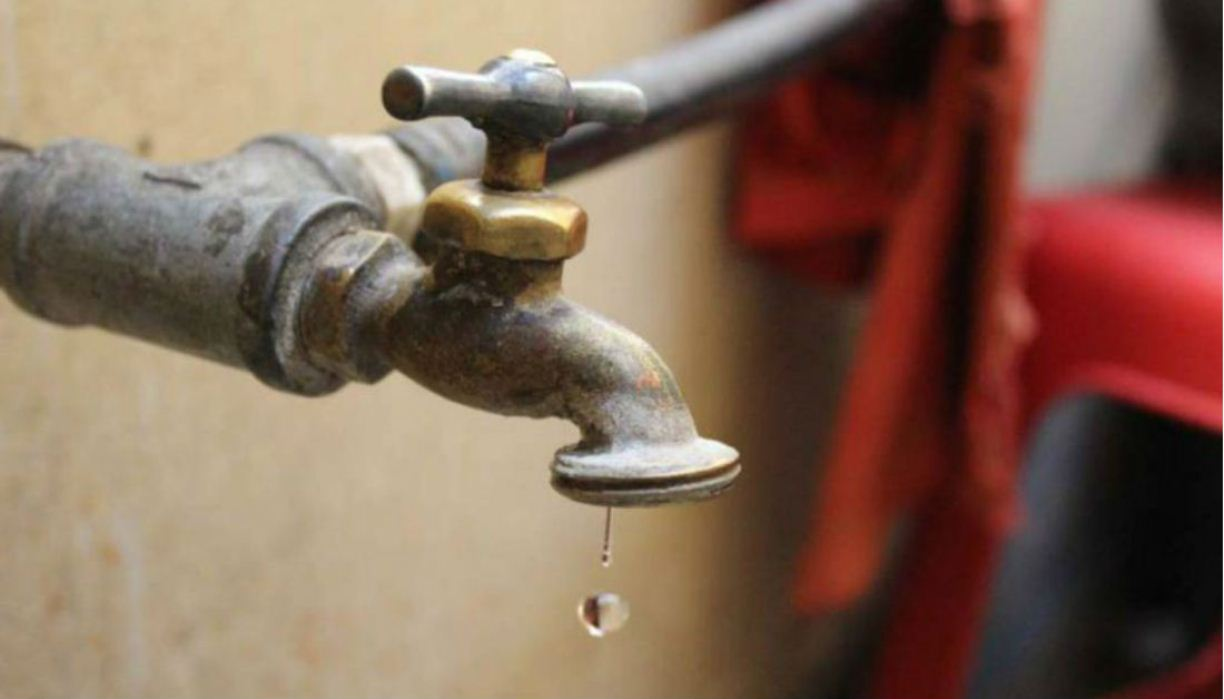
\includegraphics[width=300px]{231.jpg}%
\newline%
%
LOS TEQUES.  Más de 700 familias se ven afectadas con el plan de racionamiento que aplica Hidrocapital en el conjunto residencial Lagunetica, en la capital mirandina, donde los habitantes de 7 edificios cuentan con suministro cada 21 días, lo que desató una protesta durante la mañana este viernes que se extendió por aproximadamente 2 horas.%
\newline%
%
Comenzó como una asamblea de vecinos y posteriormente los residentes echaron mano de ramas y bolsas de basura para atravesarlas en plena vía pública y obstaculizar el paso hacia las comunidades El Trigo, Panadero, El Retén y Lagunetica, por lo que pronto conductores quedaron atascados.%
\newline%
%
“Un tanque tiene capacidad de 500 litros y si llega una vez al mes el agua no hay que ser científico para sacar la cuenta y saber que no alcanza para cubrir las necesidades básicas durante tantos días. A propósito de las circunstancias que atraviesa el país, la hidrológica anunció un plan de racionamiento, ya bastante descabellado, de 21 días de corte programado, pero la realidad es que ya van 25 días y seguimos contando”, relató Juan Martínez, vecino afectado.%
\newline%
%
Uno no puede bañarse como Dios manda, cocinar, mantener la casa limpia y lavar la ropa. Diariamente lidiamos con demasiados problemas que merman la calidad de vida. Lamentamos que los conductores queden atrapados, pero hay que llamar la atención de alguna manera. Exigimos la presencia de una comisión de Hidrocapital para reabrir la vía.%
\newline%
%
El dirigente de Voluntad Popular (VP) en el municipio Guaicaipuro, Jesús González, se ha manifestado en reiteradas ocasiones  al respecto, manifestando que la mayoría de las protestas en la zona obedecen a deficiencias en los servicios públicos.%
\newline%
%
El político expresó que la última inversión hidráulica en Venezuela se registró en el año 1981. Igualmente recalcó que desde el año 2005 hasta la fecha, al menos 12 ministros han pasado por el Ministerio del Poder Popular para Ecosocialismo y Aguas, sin solventar la situación.%
\newline%
%
La carretera Panamericana también ha sido escenario de protestas por las fallas en el suministro de agua en el municipio Los Salias, donde la suspensión de clases durante el pasado año escolar fue la constante por esta situación, problemática que proyectan se repita este período académico que recién empieza.%
\newline%
%
\end{document}